% A LaTeX (non-official) template for ISAE projects reports
% Copyright (C) 2014 Damien Roque
% Version: 0.2
% Author: Damien Roque <damien.roque_AT_isae.fr>

\documentclass[a4paper,12pt]{book}
\usepackage[utf8]{inputenc}
\usepackage[T1]{fontenc}
\usepackage[french]{babel} % If you write in French
%\usepackage[english]{babel} % If you write in English
\usepackage{a4wide}
\usepackage{graphicx}
\graphicspath{{images/}}
\usepackage{subfig}
\usepackage{tikz}
\usetikzlibrary{shapes,arrows}
\usepackage{pgfplots}
\pgfplotsset{compat=newest}
\pgfplotsset{plot coordinates/math parser=false}
\newlength\figureheight
\newlength\figurewidth
\pgfkeys{/pgf/number format/.cd,
set decimal separator={,\!},
1000 sep={\,},
}
\usepackage{ifthen}
\usepackage{ifpdf}
\ifpdf
\usepackage[pdftex]{hyperref}
\else
\usepackage{hyperref}
\fi
\usepackage{color}
\hypersetup{%
colorlinks=true,
linkcolor=black,
citecolor=black,
urlcolor=black}

\renewcommand{\baselinestretch}{1.05}
\usepackage{fancyhdr}
\pagestyle{fancy}
\fancyfoot{}
\fancyhead[LE,RO]{\bfseries\thepage}
\fancyhead[RE]{\bfseries\nouppercase{\leftmark}}
\fancyhead[LO]{\bfseries\nouppercase{\rightmark}}
\setlength{\headheight}{15pt}

\let\headruleORIG\headrule
\renewcommand{\headrule}{\color{black} \headruleORIG}
\renewcommand{\headrulewidth}{1.0pt}
\usepackage{colortbl}
\arrayrulecolor{black}

\fancypagestyle{plain}{
  \fancyhead{}
  \fancyfoot[C]{\thepage}
  \renewcommand{\headrulewidth}{0pt}
}

\makeatletter
\def\@textbottom{\vskip \z@ \@plus 1pt}
\let\@texttop\relax
\makeatother

\makeatletter
\def\cleardoublepage{\clearpage\if@twoside \ifodd\c@page\else%
  \hbox{}%
  \thispagestyle{empty}%
  \newpage%
  \if@twocolumn\hbox{}\newpage\fi\fi\fi}
\makeatother

\usepackage{amsthm}
\usepackage{amssymb,amsmath,bbm}
\usepackage{array}
\usepackage{bm}
\usepackage{multirow}
\usepackage[footnote]{acronym}

\newcommand*{\SET}[1]  {\ensuremath{\mathbf{#1}}}
\newcommand*{\VEC}[1]  {\ensuremath{\boldsymbol{#1}}}
\newcommand*{\FAM}[1]  {\ensuremath{\boldsymbol{#1}}}
\newcommand*{\MAT}[1]  {\ensuremath{\boldsymbol{#1}}}
\newcommand*{\OP}[1]  {\ensuremath{\mathrm{#1}}}
\newcommand*{\NORM}[1]  {\ensuremath{\left\|#1\right\|}}
\newcommand*{\DPR}[2]  {\ensuremath{\left \langle #1,#2 \right \rangle}}
\newcommand*{\calbf}[1]  {\ensuremath{\boldsymbol{\mathcal{#1}}}}
\newcommand*{\shift}[1]  {\ensuremath{\boldsymbol{#1}}}

\newcommand{\eqdef}{\stackrel{\mathrm{def}}{=}}
\newcommand{\argmax}{\operatornamewithlimits{argmax}}
\newcommand{\argmin}{\operatornamewithlimits{argmin}}
\newcommand{\ud}{\, \mathrm{d}}
\newcommand{\vect}{\text{Vect}}
\newcommand{\sinc}{\ensuremath{\mathrm{sinc}}}
\newcommand{\esp}{\ensuremath{\mathbb{E}}}
\newcommand{\hilbert}{\ensuremath{\mathcal{H}}}
\newcommand{\fourier}{\ensuremath{\mathcal{F}}}
\newcommand{\sgn}{\text{sgn}}
\newcommand{\intTT}{\int_{-T}^{T}}
\newcommand{\intT}{\int_{-\frac{T}{2}}^{\frac{T}{2}}}
\newcommand{\intinf}{\int_{-\infty}^{+\infty}}
\newcommand{\Sh}{\ensuremath{\boldsymbol{S}}}
\newcommand{\C}{\SET{C}}
\newcommand{\R}{\SET{R}}
\newcommand{\Z}{\SET{Z}}
\newcommand{\N}{\SET{N}}
\newcommand{\K}{\SET{K}}
\newcommand{\reel}{\mathcal{R}}
\newcommand{\imag}{\mathcal{I}}
\newcommand{\cmnr}{c_{m,n}^\reel}
\newcommand{\cmni}{c_{m,n}^\imag}
\newcommand{\cnr}{c_{n}^\reel}
\newcommand{\cni}{c_{n}^\imag}
\newcommand{\tproto}{g}
\newcommand{\rproto}{\check{g}}
\newcommand{\LR}{\mathcal{L}_2(\SET{R})}
\newcommand{\LZ}{\ell_2(\SET{Z})}
\newcommand{\LZI}[1]{\ell_2(\SET{#1})}
\newcommand{\LZZ}{\ell_2(\SET{Z}^2)}
\newcommand{\diag}{\operatorname{diag}}
\newcommand{\noise}{z}
\newcommand{\Noise}{Z}
\newcommand{\filtnoise}{\zeta}
\newcommand{\tp}{g}
\newcommand{\rp}{\check{g}}
\newcommand{\TP}{G}
\newcommand{\RP}{\check{G}}
\newcommand{\dmin}{d_{\mathrm{min}}}
\newcommand{\Dmin}{D_{\mathrm{min}}}
\newcommand{\Image}{\ensuremath{\text{Im}}}
\newcommand{\Span}{\ensuremath{\text{Span}}}

\newtheoremstyle{break}
  {11pt}{11pt}%
  {\itshape}{}%
  {\bfseries}{}%
  {\newline}{}%
\theoremstyle{break}

%\theoremstyle{definition}
\newtheorem{definition}{Définition}[chapter]

%\theoremstyle{definition}
\newtheorem{theoreme}{Théorème}[chapter]

%\theoremstyle{remark}
\newtheorem{remarque}{Remarque}[chapter]

%\theoremstyle{plain}
\newtheorem{propriete}{Propriété}[chapter]
\newtheorem{exemple}{Exemple}[chapter]

\parskip=5pt
%\sloppy

\begin{document}

%%%%%%%%%%%%%%%%%%
%%% First page %%%
%%%%%%%%%%%%%%%%%%

\begin{titlepage}
\begin{center}


\includegraphics[width=0.6\textwidth]{logo-isae-supaero}\\[1cm]

{\large Rapport de Stage de fin d'étude}\\[0.5cm]

{\large ACCOU Martin}\\[0.5cm]

% Title
\rule{\linewidth}{0.5mm} \\[0.4cm]
{ \huge \bfseries Titre \\[0.4cm] }
\rule{\linewidth}{0.5mm} \\[1.5cm]


\vfill

% Bottom of the page
{\large Version 0.1 du\\ \today}

\end{center}
\end{titlepage}

%%%%%%%%%%%%%%%%%%%%%%%%%%%%%
%%% Non-significant pages %%%
%%%%%%%%%%%%%%%%%%%%%%%%%%%%%

\frontmatter

\clearpage
\tableofcontents

\clearpage
\listoffigures

\clearpage

%%%%%%%%%%%%%%%%%%%%%%%%%%%%%%%%%%%%%%%%%%%%
%%% Content of the report and references %%%
%%%%%%%%%%%%%%%%%%%%%%%%%%%%%%%%%%%%%%%%%%%%

\mainmatter
\pagestyle{fancy}

\cleardoublepage

\chapter{Introduction}
\addcontentsline{toc}{chapter}{Introduction}
\markboth{Introduction}{Introduction}
\label{chap:introduction}
%\minitoc

%%% Local Variables: 
%%% mode: latex
%%% TeX-master: "isae-report-template"
%%% End: 

\section{D3S, a leader in 3D CAD Analytics}

D3S, which stands for Data Science Softwares \& Services, specializes in delivering customized software solutions utilizing AI technologies. The company comprises a team of Data Scientists and Full Stack Developers with deep expertise in 3D CAD (Computer-Aided Design) Analytics and Natural Language Processing (NLP).  

Its state-of-the-art technologies are built on open-source libraries and supported by internal R\&D, enabling efficient data extraction through computer vision, Optical Character Recognition (OCR), and NLP. D3S also excels in deep learning applications such as 3D morpho analysis, metrics comparison, BoM (Bill of Materials) analytics, and time series processing. 

The company’s solutions are designed to provide scalable, adaptable, and secure business value for industries like aerospace and automotive.

\vspace{0.5cm}

I have been working with the 3D CAD Analytics team, where my focus was on developing a 3D similarity model designed to compare CAD designs solely based on their geometric properties.

\begin{figure}[]
    \centering
    
\includegraphics[width=0.3\columnwidth]{images/d3s_logo.png}
    \caption{D3S, Data Science Softwares \& Services}
    \label{fig:d3s_logo}
\end{figure}

\section{3D similarity model}

3D model designers spend a significant amount of time searching for relevant information during the product design process, even though much of their work could be done by modifying existing Computer-Aided Design (CAD) designs. As a result, the retrieval and reuse of CAD designs are crucial in CAD design management. However, large CAD design repositories often require extensive categorization or organization of engineering data, making design reuse challenging. Traditionally, the classification and retrieval of 3D CAD designs involved a manual process of labeling, which is time-consuming, prone to errors, and inefficient. This issue becomes even more pronounced when designs are generated in product development, as inconsistent labeling and tagging across different systems lead to the complex task of data harmonization. Additionally, the inherent complexity of 3D CAD design definitions makes it difficult to apply rigid, general classification rules, as design features and parameters vary depending on their origin. Therefore, an automated approach to classification and retrieval is needed to address these challenges.

The goal is to automatically associate a given design to similar other designs, as depicted in \autoref{fig:similar-designs}. This will make it possible to leverage the D3S dataset of industrial 3D designs, in order to infer missing information, such as the name of a design, its function, or its material.

\begin{figure}[]
    \centering
    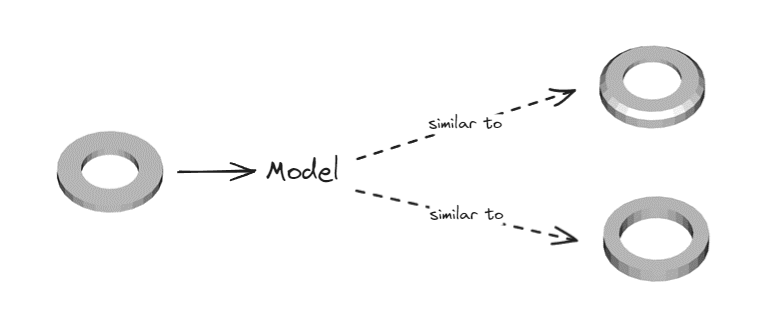
\includegraphics[width=0.8\columnwidth]{images/similar-pieces.png}
    \caption{Purpose of our similarity model}
    \label{fig:similar-designs}
\end{figure}

In recent years, point cloud representations has become one of the research hotspots in the field of computer vision \cite{zhangDeepLearningbased3D2023}.
In our case, we can not directly train a powerful classifier, because of a lack of clean labeled data and of the variety of the possible 3D designs.
The most comprehensive dataset available consists of just 2,000 CAD designs, with rather imprecise labeling. Examples of labels include coupling strap, shackle, and long beam. It is evident that there is a significant need for a more curated and accurate dataset in this area, which is really hard to obtain.

Given the recent success of self-supervised learning methods, more specifically contrastive learning \cite{radfordLearningTransferableVisual2021,yuPointBERTPretraining3D2022,liuOpenShapeScaling3D2023}, an innovative and promising approach has been proposed to tackle this problem.

The goal is to learn a representation of data such that similar instances are close together in the representation space, while dissimilar instances are far apart. To do so, a triplet loss, popularized by the FaceNet model \cite{schroffFaceNetUnifiedEmbedding2015}, will be used. Since we lack labeled data, we can't generate triplets directly as in \cite{schroffFaceNetUnifiedEmbedding2015}. Instead, a 'Tinder-like' application has been developped and used by the whole company to build our labeled triplets database. To clarify, a labeled triplet consists of three 3D models: an anchor, a positive, and a negative model. The detailed framework of our triplet loss is outlined in \autoref{sec:triplet-loss-training}. In this setup, the anchor and positive models are similar to each other, whereas the negative model is distinct from both.

To summarize, the pipeline comprises the two main following steps:
\begin{enumerate}
    \item \textbf{Triplets collection}: Offline unlabeled triplets are generated. Triplets are then labeled by the users of the app and stored in the database.
    \item \textbf{Model training}: An encoding model is trained on the labeled triplets. The model is then used to compute the similarity between two 3D designs.
\end{enumerate}

\begin{figure}[]
    \centering
    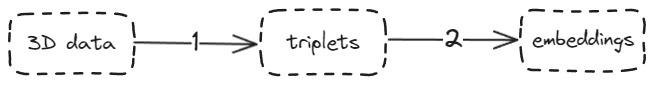
\includegraphics[width=0.8\columnwidth]{images/steps.png}
    \caption{Pipeline for building the model}   
    \label{fig:steps}
\end{figure}
\chapter{Related work}
\label{chap:related_work}

\section{3D Understanding}

3D data can be presented in various formats, and the selection of the format is critical and depends on the specific needs of the application. A CAD model is a 3D representation of a physical object. At a higher level, the Standard for the Exchange of Product model data (STEP format) is a widely adopted ISO standard for data exchange that can represent 3D objects in CAD and related information. In this format, a CAD model is defined by its topological components such as faces, edges, or vertices and the connections between them. At a lower level, the STL format is a file format that represents 3D objects as a collection of triangles (mesh). This format is commonly used in 3D printing and computer graphics. Additionally, the point cloud format consists of a set of points in a 3D space, with each point representing a single point on the surface of the object. This format can be easily derived from an STL file by sampling points on the mesh surface. Other formats worth mentioning include voxel and multi-view image formats \cite{zhangDeepLearningbased3D2023}.

The decision was made to explore both STL and point cloud formats. The choice of the STL format is driven by its widespread use in the industry and the ease of generating a point cloud from it. Notably, models based on the STEP format \cite{mandelliCAD3DModel2022}, while promising, were not considered because they limit the scope too much.

Following recent trends in the field, two main classes of models were investigated, graph-based models and transformer-based models.

\subsubsection{Graph-based models}

Graph neural networks (GNN) have been used recently in numerous applications \cite{wuComprehensiveSurveyGraph2021,jumperHighlyAccurateProtein2021}
The flexible nature of a graph permits its usage from data sets concerning large social networks to smaller networks that describe the chemical bonds of a molecule. Graph neural networks use the correspondences between elements instead of focusing on individual elements. These correspondences help create neighborhoods and local regions, which greatly enhance the predictive accuracy of the resulting features.

Given an input mesh, a natural candidate is a graph which nodes are the vertices of the mesh and where each vertex is connected to the vertices that share a face with it. This information is not available for the different GNNs that have been developed for 3D point cloud data \cite{vermaFeaStNetFeatureSteeredGraph2018,wangDynamicGraphCNN2019,dengPPFNetGlobalContext2018}. These models are designed to work with point clouds. The main challenge is to define a graph structure that captures the local and global features of the point cloud. The most common approach is to define a graph where each point is a node and the edges are defined by the k-nearest neighbors of each point. The graph is then fed to a GNN to extract features from the point cloud.

\subsubsection{Transformer-based models}
Transformers \cite{vaswaniAttentionAllYou2023b} and self-attention models have revolutionized machine translation and natural language processing. 
They can equal or even surpass convolutional networks when applied to sequences and 2D images \cite{dosovitskiyImageWorth16x162021}. 

Self-attention is especially relevant in our context, as it naturally functions as a set operator, where positional information is treated as an attribute of elements within a set. Given that 3D point clouds consist of sets of points with positional attributes, the self-attention mechanism appears particularly well-suited to handling this type of data. Many recent works have explored the application of transformers to 3D data \cite{zhaoPointTransformer2021,yuPointBERTPretraining3D2022,liuOpenShapeScaling3D2023}.


\section{Contrastive learning}


%%% Local Variables: 
%%% mode: latex
%%% TeX-master: "isae-report-template"
%%% End: 
\chapter{Method}
\label{sec:method}

We propose a method for constructing a similarity model from an unlabeled dataset that contains a small proportion of approximately labeled instances. This method is applied on our use case of 3D CAD designs, but it is actually generalizable to other domains. 

Unlabeled triplets are generated from the entire dataset \autoref{sec:triplet-generation}. These triplets are then labeled using a dedicated application \autoref{sec:labeling-application}. Finally, the labeled triplets are used to train a model based on triplet loss \autoref{sec:triplet-loss-training}.


\section{Labeling application}
\label{sec:labeling-application}

Before delving into the details of the pipeline, it is essential to introduce the user interface that has been developed in order to build the labeled triplets database.

There are actually two main use cases for the application: labeling triplets (\autoref{fig:labeling_use_case}) and comparing two iterations of a model (\autoref{fig:validation_use_case}).

\begin{itemize}
  \item \textbf{Labeling triplets:} Users are presented with a triplet of 3D designs, with the reference design (anchor) in the center. Their task is to swipe left or right to indicate whether the left or right design is more similar to the anchor design. A skip option is also available for ambiguous cases.
  
  Users can also change to a canonical view of the designs to facilitate the comparison. This changes the perspective of a camera to a view aligned with the design's principal axes. This may or may not be useful depending on the design's geometry, as shown in \autoref{fig:default_vs_canonical}.

\begin{figure}[]
  \centering
  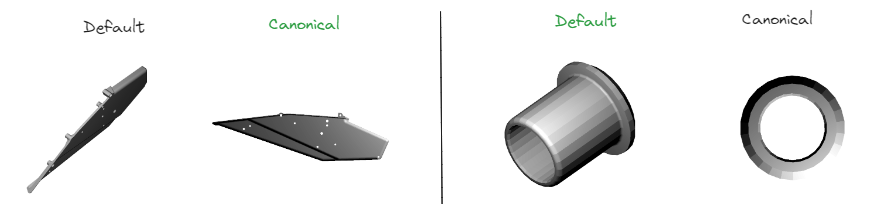
\includegraphics[width=\columnwidth]{images/default_vs_canonical.png}
  \caption{Two designs where the appropriate view is different.}
  \label{fig:default_vs_canonical}
\end{figure}

  Additional metadata is also provided to the users, such as the design length. This information can help users make more informed decisions when the geometry does not suffice.
  \item \textbf{Validation:} A similar interface is used, but now the propositions on the left and right are two nearest neighbors propositions of two different designs. Users judge which model gives the best nearest neighbor proposition. This gives an easy way to compare two iterations of a model. This is especially useful to bulletproof the model's performance, ensuring robustness not only in quantitative metrics but also in qualitative assessments.
  
\end{itemize}

\begin{figure}[]
  \centering
  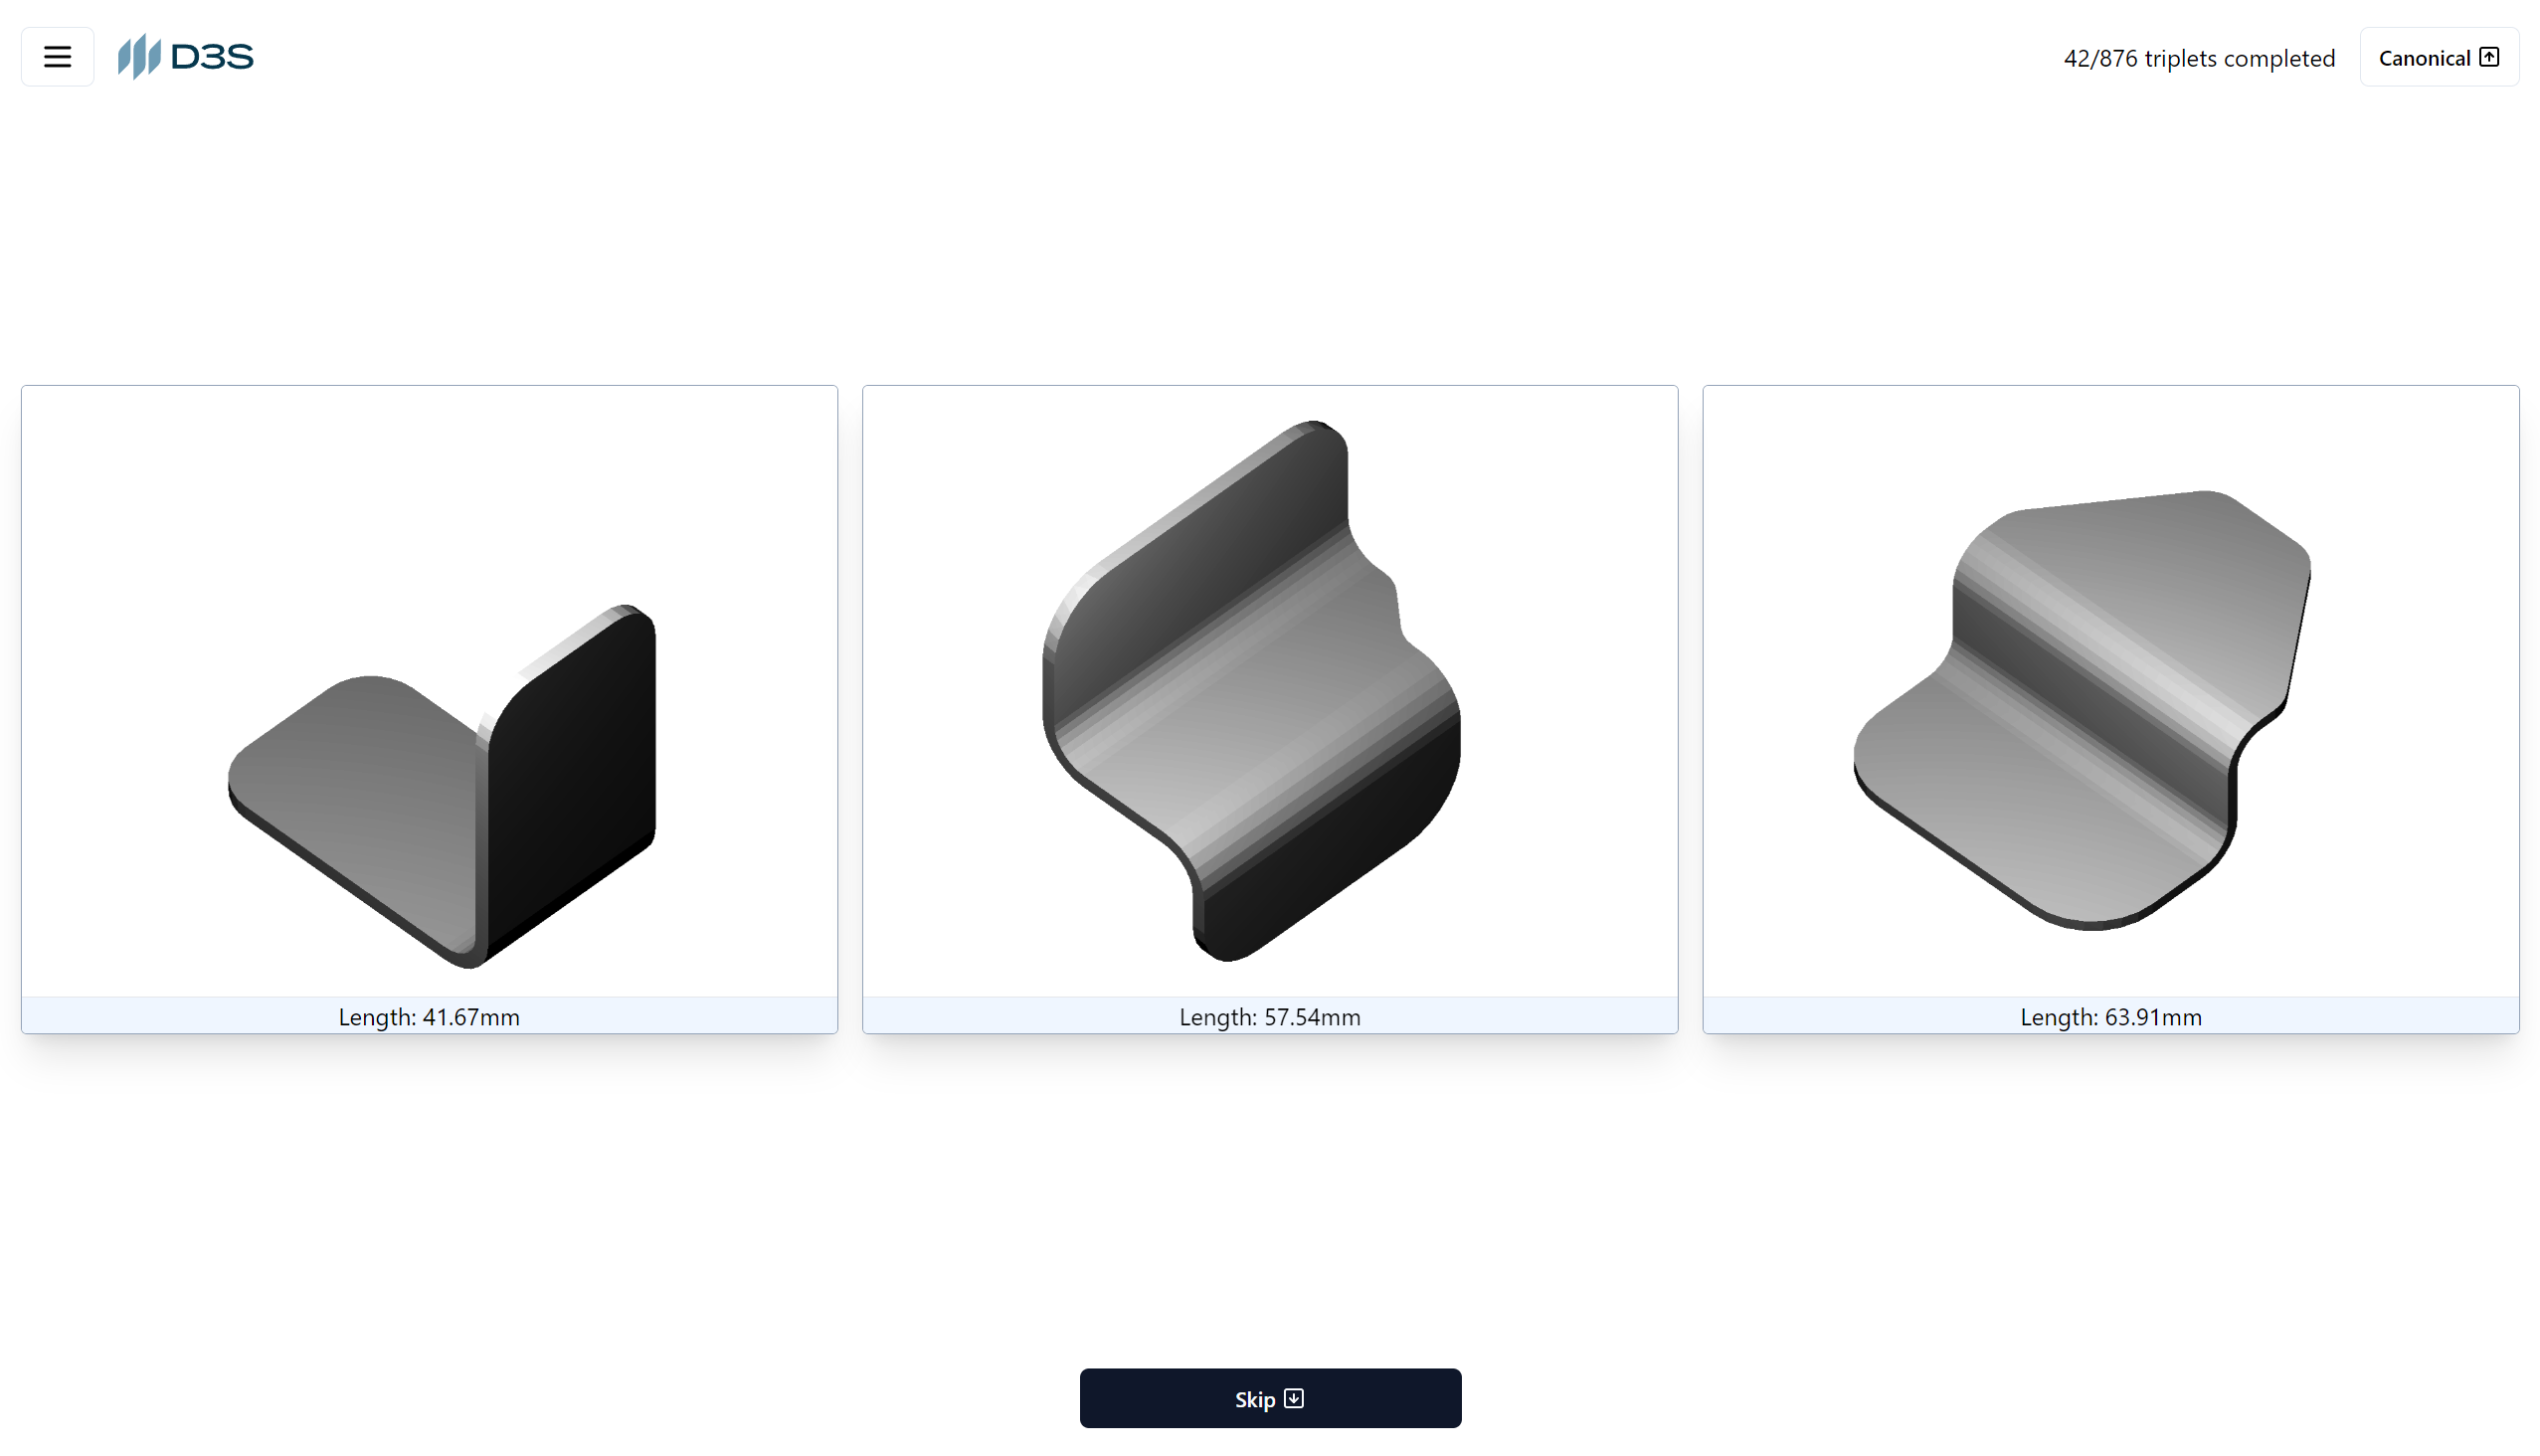
\includegraphics[width=0.8\columnwidth]{images/tinder3d_labeling.png}
  \caption{User interface for the labeling use case. Here, the design on the right is more similar to the anchor design in the center (curved edges).}
  \label{fig:labeling_use_case}
\end{figure}

\begin{figure}[]
  \centering
  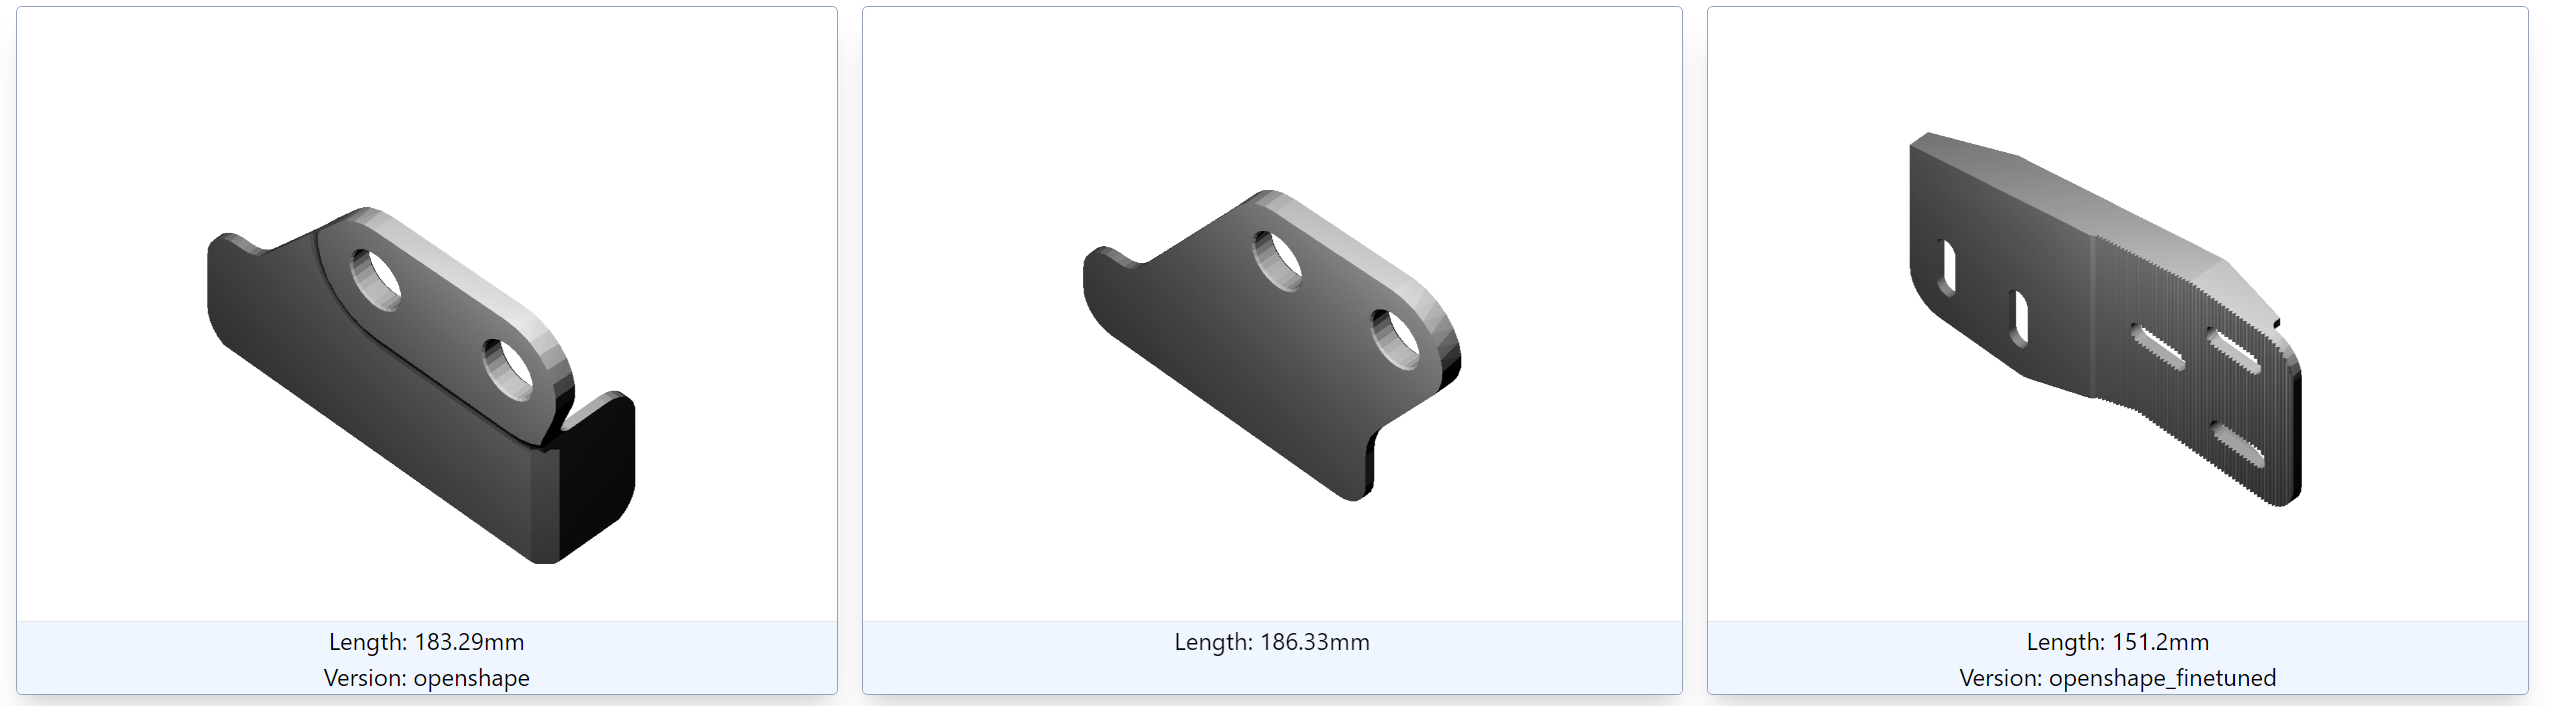
\includegraphics[width=0.8\columnwidth]{images/tinder3d_validation.png}
  \caption{User interface for the validation use case. Here, the proposition of the model on the left is more similar to the anchor design in the center (two holes at the top).}
  \label{fig:validation_use_case}
\end{figure}

This application is designed to be intuitive and user-friendly, allowing users to quickly and efficiently label triplets.

Additional gamification elements were considered at one point, but they were deemed unnecessary as we were already achieving strong results with a small number of triplets.

\section{Triplet loss training}
\label{sec:triplet-loss-training}

The goal is to learn a representation of data such that similar instances are close together in the representation space, while dissimilar instances are far apart. We are going to use a triplet loss approach to train our encoder model. Once we will have our embeddings, the \textbf{cosine similarity} will be used to define a distance among the data points.

$$d(x, y) = 1 - \frac{x \cdot y}{\|x\| \|y\|}$$

The loss will be defined over triplets of embeddings:
\begin{itemize}
  \item An anchor.
  \item A positive, of the same class as the anchor.
  \item A negative, of a different class than the anchor.
\end{itemize}

\vspace{0.2cm}

Given a batch size $N$, a distance function $d$, a margin $margin$ and $a$, $p$ and $n$ tensors representing anchor, positive and negative examples, respectively.

$\ell(a, p, n)=L=\left\{l_1, \ldots, l_N\right\}^{\top}, \quad l_i=\max \left\{d\left(a_i, p_i\right)-d\left(a_i, n_i\right)+\text { margin }, 0\right\}$

Input tensors $a$, $p$ and $n$ are of shape $(N, D)$, where $D$ is the embedding dimension. The loss $l_i$ is computed for each triplet in the batch, and the final loss is the mean of all individual losses.

Intuitively, you aim to group the data into separate clusters, ensuring that each class forms its own cluster. However, the precise distance between clusters isn't a concern, as long as they remain clearly distinct. Without limiting the loss, the model could improve by pushing an easy negative example very far away, while neglecting more challenging negative examples. By capping the reward beyond a certain distance, the model is encouraged to focus on the harder examples to continue improving.

Based on the definition of the loss, there are three categories of triplets:
\begin{itemize}
  \item \textbf{Easy triplets:} Triplets which have a loss of $0$, because $d(a, p) + margin < d(a, n)$.
  \item \textbf{Hard triplets:} Triplets where the negative is closer to the anchor than the positive, i.e. $d(a, n) < d(a, p)$.
  \item \textbf{Semi-hard triplets:} Triplets where the negative is not closer to the anchor than the positive, but which still have positive loss: $d(a, p) < d(a, n) < d(a, p) + margin$.
\end{itemize}

\begin{figure}[]
  \centering
  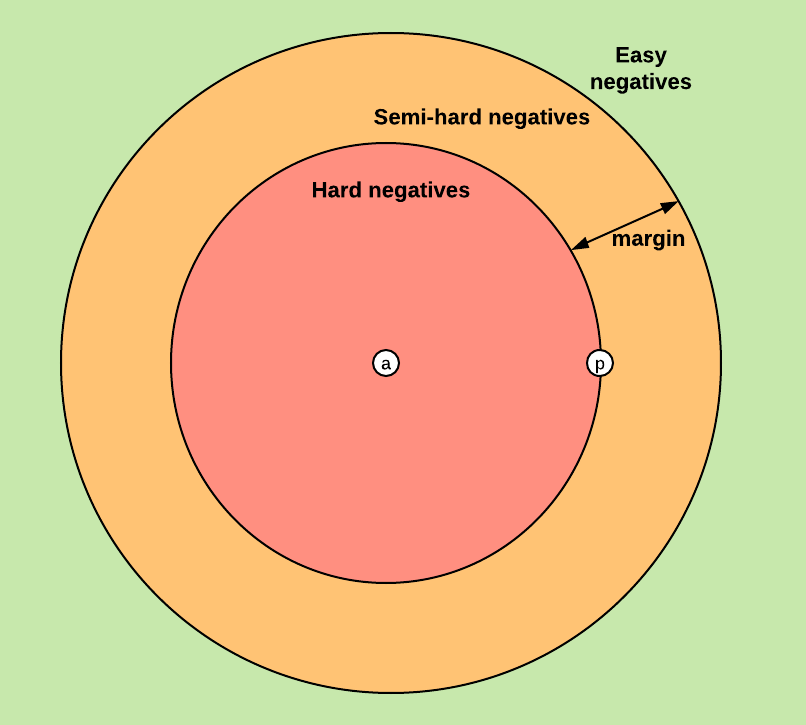
\includegraphics[width=0.5\columnwidth]{images/negative_types.png}
  \caption{The three types of negatives, given an anchor and a positive.}
  \label{fig:negative_types}
\end{figure}

The balance of these triplet types is crucial for the model's performance, as we will see in TODO.

Before delving deeper into working on triplet loss, we had to first ensure that training a triplet loss model with 'fake triplets' generated from our labeled dataset yielded similar results to a classification model trained on the same dataset. To do so, a GNN based on the EdgeConv architecure \cite{wangDynamicGraphCNN2019} was used. 

The performance of the classification model was evaluated against the triplet loss model using a nearest neighbor approach. This method assessed how often a design's label matched that of its closest neighbor in the learned representation space. Both models achieved a 95\% accuracy rate, suggesting that the triplet loss model successfully learned to create meaningful representations of the data. It is important to emphasize that at this point only triplets generated from the labels were used, and no human labeling was done. Triplets are generated following the same approach as in \autoref{sec:triplet-generation-heuristics}, but ensuring that the anchor and the positive are indeed of the same class. 

With just 1000 triplets, the model achieved a nearest neighbor accuracy similar to the classification model. However, optimal performance was observed when using approximately 10000 triplets, which resulted in a 95\% accuracy rate.

\section{Triplets generation}
\label{sec:triplet-generation}

There is still the question of how to generate the triplets that are going to be labeled by the user of the app. Let's draw the properties of the triplets we want to generate, ordered by ease of implementation:
\begin{enumerate}
  \item The triplets should be diverse enough to cover the entire dataset.
  \item Almost every triplet should be 'labelable'. A triplet is 'labelable' if users do not have to skip it. This is a mainly a user experience concern. 
  \item A great proportion of triplets should be 'hard triplets' for the model that generated them, ie triplets where the negative is hard. This will force the next iteration of the model to learn from its misconceptions.
\end{enumerate}


A simple yet effective way has been proposed to generate triplets. For the initial generation, a model trained on the small labeled dataset we had was used to compute embeddings for the entire dataset. This model was used to generate triplets based on heuristics which are detailed in \autoref{sec:triplet-generation-heuristics}. Subsequently, the model was retrained on the labeled triplets, and the process was repeated iteratively.

With such a method, property 1 is straightforward to achieve, as a random selection of triplets will cover the entire dataset. Property 2 and 3 are in conflict, as a triplet that is easy to label is likely to be easy for the model as well. Considering the limits, selecting candidates that are equidistant from the anchor is intriguing, but tends to result in many 'skipped' triplets. Conversely, choosing candidates where the first is closer than the second will lead to fewer skipped triplets, but also a lower proportion of semi-hard and hard triplets.

It's why a proper balance has to be found, as explained in \autoref{sec:triplet-generation-heuristics}.

%%% Local Variables: 
%%% mode: latex
%%% TeX-master: "isae-report-template"
%%% End: 
\chapter{Un chapitre}
\label{sec:unchapitre}

Lorem ipsum dolor sit amet, consectetur adipiscing elit. Sed non risus. Suspendisse lectus tortor, dignissim sit amet, adipiscing nec, ultricies sed, dolor. Cras elementum ultrices diam. Maecenas ligula massa, varius a, semper congue, euismod non, mi. Proin porttitor, orci nec nonummy molestie, enim est eleifend mi, non fermentum diam nisl sit amet erat. Duis semper. Duis arcu massa, scelerisque vitae,  convallis sollicitudin purus. Praesent aliquam, enim at fermentum mollis, ligula massa adipiscing nisl, ac euismod nibh nisl eu lectus. Fusce vulputate sem at sapien. Vivamus leo. Aliquam euismod libero eu enim. Nulla nec felis sed leo placerat imperdiet. Aenean suscipit nulla in justo. Suspendisse cursus rutrum augue. Nulla tincidunt tincidunt mi. Curabitur iaculis, lorem vel rhoncus faucibus, felis magna fermentum augue, et ultricies lacus lorem varius purus. Curabitur eu amet. Encore une citation \cite{Cadambe2008}.

\begin{figure}[htp!]
  \centering
  \setlength\figureheight{7cm}
  \setlength\figurewidth{9cm}
  % This file was created by matlab2tikz v0.2.2.
% Copyright (c) 2008--2012, Nico Schlömer <nico.schloemer@gmail.com>
% All rights reserved.
% 
% 
% 

% defining custom colors
\definecolor{mycolor1}{rgb}{0,0.75,0.75}

\begin{tikzpicture}

\begin{axis}[%
view={0}{90},
width=\figurewidth,
height=\figureheight,
scale only axis,
xmin=2, xmax=4.5,
xlabel={$\eta$},
xmajorgrids,
ymin=0.5, ymax=1,
ylabel={$d_{\text{min}}^2$},
ymajorgrids,
legend cell align=left,
legend style={align=left}]
\addplot [
color=black,
dashed,
mark=asterisk,
mark options={solid}
]
coordinates{
 (2,1)(2.1,1)(2.2,1)(2.3,1)(2.4,1)(2.5,1)(2.6,0.937749781479547)(2.7,0.890900393128398)(2.8,0.864988513955105)(2.9,0.827013168393703)(3,0.811347612650328)(3.1,0.792559278041243)(3.2,0.765840563467819)(3.3,0.749680961469385)(3.4,0.741947149227874)(3.5,0.740609493518419)(3.6,0.732128087463441)(3.7,0.717775843626632)(3.8,0.699687461812158)(3.9,0.685018622769455)(4,0.673439611642851)(4.1,0.664624248264608)(4.2,0.658255928882634)(4.3,0.641702335270489)(4.4,0.608326504614558)(4.5,0.580489221369454) 
};
\addlegendentry{$\alpha\text{ =  0\%}$};

\addplot [
color=black,
dashed,
mark=x,
mark options={solid}
]
coordinates{
 (2,1)(2.1,1)(2.2,1)(2.3,1)(2.4,0.958561324724996)(2.5,0.900812804739278)(2.6,0.859608621629443)(2.7,0.828484932127753)(2.8,0.812298837741994)(2.9,0.778916291864501)(3,0.758500630955482)(3.1,0.748375165853317)(3.2,0.745960208532468)(3.3,0.738441167434538)(3.4,0.715506361296671)(3.5,0.696927131434508)(3.6,0.682276848692725)(3.7,0.671128156410174)(3.8,0.663062783265717)(3.9,0.657680299791254)(4,0.621142740976429)(4.1,0.589786339121755)(4.2,0.564530571776849)(4.3,0.54483432747474)(4.4,0.53008799514765)(4.5,0.519641830384595) 
};
\addlegendentry{$\alpha\text{ = 10\%}$};

\addplot [
color=black,
dashed,
mark=triangle,
mark options={solid}
]
coordinates{
 (2,1)(2.1,1)(2.2,1)(2.3,0.966145915091813)(2.4,0.907589260275562)(2.5,0.862273165052718)(2.6,0.833762738286283)(2.7,0.797262289343802)(2.8,0.774689700869446)(2.9,0.763077871790574)(3,0.759584455148894)(3.1,0.735410358863577)(3.2,0.713220246811223)(3.3,0.695713299974315)(3.4,0.682371019886023)(3.5,0.672682085917092)(3.6,0.6661550402729)(3.7,0.644666127799479)(3.8,0.610083129739041)(3.9,0.582172698611821)(4,0.560333265725228)(4.1,0.543883933286703)(4.2,0.532098369213191)(4.3,0.524242326405)(4.4,0.519608701974017)(4.5,0.517545187250875) 
};
\addlegendentry{$\alpha\text{ = 20\%}$};

\addplot [
color=black,
dashed,
mark=triangle,
mark options={solid,,rotate=180}
]
coordinates{
 (2,1)(2.1,1)(2.2,0.995488894312993)(2.3,0.930050749246739)(2.4,0.882604857341179)(2.5,0.840148695151764)(2.6,0.807621264874927)(2.7,0.787889977099099)(2.8,0.777972678915356)(2.9,0.750463202108443)(3,0.726620292578349)(3.1,0.707917379352703)(3.2,0.693763185722015)(3.3,0.683575144048861)(3.4,0.676795290182409)(3.5,0.663350261880571)(3.6,0.627666127013326)(3.7,0.598755039468926)(3.8,0.575986310488554)(3.9,0.558651995817327)(4,0.546003746104731)(4.1,0.537291509323841)(4.2,0.531798375059385)(4.3,0.528867181690889)(4.4,0.527917002741411)(4.5,0.528450017604181) 
};
\addlegendentry{$\alpha\text{ = 30\%}$};

\addplot [
color=black,
dashed,
mark=o,
mark options={solid}
]
coordinates{
 (2,1)(2.1,1)(2.2,1)(2.3,1)(2.4,1)(2.5,0.995096871086856)(2.6,0.937749790013923)(2.7,0.890900391028178)(2.8,0.864988509535523)(2.9,0.827013167946275)(3,0.811347609462027)(3.1,0.79255927917077)(3.2,0.765840564829299)(3.3,0.749680963181722)(3.4,0.741947149533667)(3.5,0.740609492450166)(3.6,0.732128080624777)(3.7,0.71777584554089)(3.8,0.699687463368726)(3.9,0.681193180471954)(4,0.640212533267028)(4.1,0.617585040920557)(4.2,0.608519007405809)(4.3,0.608298095410932)(4.4,0.608326494076335)(4.5,0.580489212682311) 
};
\addlegendentry{Mazo};

\end{axis}
\end{tikzpicture}%
  \caption{Exemple de courbe TikZ.}
  \label{fig:courbe-tikz}
\end{figure}

\section{Analyse aux limites}
Lorem ipsum dolor sit amet, consectetur adipiscing elit. Sed non risus. Suspendisse lectus tortor, dignissim sit amet, adipiscing nec, ultricies sed, dolor. Cras elementum ultrices diam. Maecenas ligula massa, varius a, semper congue, euismod non, mi. Proin porttitor, orci nec nonummy molestie, enim est eleifend mi, non fermentum diam nisl sit amet erat. Duis semper. Duis arcu massa, scelerisque vitae, consequat in, pretium a, enim. Pellentesque congue. Ut in risus volutpat libero pharetra tempor. Cras vestibulum bibendum augue. Praesent egestas leo in pede. Praesent blandit odio eu enim. Pellentesque sed dui ut augue blandit sodales. Vestibulum ante ipsum primis in faucibus orci luctus et ultrices posuere cubilia Curae; Aliquam nibh. Mauris ac mauris sed pede pellentesque fermentum. Maecenas adipiscing ante non diam sodales hendrerit. Ut velit mauris, egestas sed, gravida nec, ornare ut, mi. Aenean ut orci vel massa suscipit pulvinar. Nulla sollicitudin. Fusce varius, ligula non tempus aliquam, nunc turpis ullamcorper nibh, in tempus sapien eros vitae ligula. Pellentesque rhoncus nunc et augue. Integer id felis. Curabitur aliquet pellentesque diam. Integer quis metus vitae elit lobortis egestas. Lorem ipsum dolor sit amet, consectetuer adipiscing elit. Morbi vel erat non mauris convallis vehicula. Nulla et sapien. Integer tortor tellus, aliquam faucibus, convallis id, congue eu, quam. Mauris ullamcorper felis vitae erat. Proin feugiat, augue non elementum posuere, metus purus iaculis lectus, et tristique ligula justo vitae magna. Aliquam convallis sollicitudin purus. Praesent aliquam, enim at fermentum mollis, ligula massa adipiscing nisl, ac euismod nibh nisl eu lectus. Fusce vulputate sem at sapien. Vivamus leo. Aliquam euismod libero eu enim. Nulla nec felis sed leo placerat imperdiet. Aenean suscipit nulla in justo. Suspendisse cursus rutrum augue. Nulla tincidunt tincidunt mi. Curabitur iaculis, lorem vel rhoncus faucibus, felis magna fermentum augue, et ultricies lacus lorem varius purus. Curabitur eu amet.

\subsection{Quelques détails sur cette méthode}
Lorem ipsum dolor sit amet, consectetuer adipiscing elit. Morbi vel erat non mauris convallis vehicula. Nulla et sapien. Integer tortor tellus, aliquam faucibus, convallis id, congue eu, quam. Mauris ullamcorper felis vitae erat. Proin feugiat, augue non elementum posuere, metus purus iaculis lectus, et tristique ligula justo vitae magna. Aliquam convallis sollicitudin purus. Praesent aliquam, enim at fermentum mollis, ligula massa adipiscing nisl, ac euismod nibh nisl eu lectus. Fusce vulputate sem at sapien. Vivamus leo. Aliquam euismod libero eu enim. Nulla nec felis sed leo placerat imperdiet. Aenean suscipit nulla in justo. Suspendisse cursus rutrum augue. Nulla tincidunt tincidunt mi. Curabitur iaculis, lorem vel rhoncus faucibus, felis magna fermentum augue, et ultricies lacus lorem varius purus. Curabitur eu amet.

\subsection{On n'est jamais très fort pour ce calcul}
Lorem ipsum dolor sit amet, consectetuer adipiscing elit. Morbi vel erat non mauris convallis vehicula. Nulla et sapien. Integer tortor tellus, aliquam faucibus, convallis id, congue eu, quam. Mauris ullamcorper felis vitae erat. Proin feugiat, augue non elementum posuere, metus purus iaculis lectus, et tristique ligula justo vitae magna. Aliquam convallis sollicitudin purus. Praesent aliquam, enim at fermentum mollis, ligula massa adipiscing nisl, ac euismod nibh nisl eu lectus. Fusce vulputate sem at sapien. Vivamus leo. Aliquam euismod libero eu enim. Nulla nec felis sed leo placerat imperdiet. Aenean suscipit nulla in justo. Suspendisse cursus rutrum augue. Nulla tincidunt tincidunt mi. Curabitur iaculis, lorem vel rhoncus faucibus, felis magna fermentum augue, et ultricies lacus lorem varius purus. Curabitur eu amet.

\begin{align}
H_{m,n,p,q} &= \DPR{\rproto_{p,q}}{\OP{H} \tproto_{m,n}}\\
&= \iint\limits_{\SET{R}^2} S_{\OP{H}}(f,\tau) \DPR{\rproto_{p,q}}{\OP{U}_{f,\tau} \tproto_{m,n}} \ud f \ud \tau.
\end{align}

\section{Vérification par simulation numérique}
Lorem ipsum dolor sit amet, consectetur adipiscing elit. Sed non risus. Suspendisse lectus tortor, dignissim sit amet, adipiscing nec, ultricies sed, dolor. Cras elementum ultrices diam. Maecenas ligula massa, varius a, semper congue, euismod non, mi. Proin porttitor, orci nec nonummy molestie, enim est eleifend mi, non fermentum diam nisl sit amet erat. Duis semper. Duis arcu massa, scelerisque vitae, consequat in, pretium a, enim. Pellentesque congue. Ut in risus volutpat libero pharetra tempor. Cras vestibulum bibendum augue. Praesent egestas leo in pede. Praesent blandit odio eu enim. Pellentesque sed dui ut augue blandit sodales. Vestibulum ante ipsum primis in faucibus orci luctus et ultrices posuere cubilia Curae; Aliquam nibh. Mauris ac mauris sed pede pellentesque fermentum. Maecenas adipiscing ante non diam sodales hendrerit. Ut velit mauris, egestas sed, gravida nec, ornare ut, mi. Aenean ut orci vel massa suscipit pulvinar. Nulla sollicitudin. Fusce varius, ligula non tempus aliquam, nunc turpis ullamcorper nibh, in tempus sapien eros vitae ligula. Pellentesque rhoncus nunc et augue. Integer id felis. Curabitur aliquet pellentesque diam. Integer quis metus vitae elit lobortis egestas. Lorem ipsum dolor sit amet, consectetuer adipiscing elit. Morbi vel erat non mauris convallis vehicula. Nulla et sapien. Integer tortor tellus, aliquam faucibus, convallis id, congue eu, quam. Mauris ullamcorper felis vitae erat. Proin feugiat, augue non elementum posuere, metus purus iaculis lectus, et tristique ligula justo vitae magna. Aliquam convallis sollicitudin purus. Praesent aliquam, enim at fermentum mollis, ligula massa adipiscing nisl, ac euismod nibh nisl eu lectus. Fusce vulputate sem at sapien. Vivamus leo. Aliquam euismod libero eu enim. Nulla nec felis sed leo placerat imperdiet. Aenean suscipit nulla in justo. Suspendisse cursus rutrum augue. Nulla tincidunt tincidunt mi. Curabitur iaculis, lorem vel rhoncus faucibus, felis magna fermentum augue, et ultricies lacus lorem varius purus. Curabitur eu amet.

%%% Local Variables: 
%%% mode: latex
%%% TeX-master: "isae-report-template"
%%% End: 
\chapter*{Conclusion}
\addcontentsline{toc}{chapter}{Conclusion}
\markboth{Conclusion}{Conclusion}
\label{sec:conclusion}

    Lorem ipsum dolor sit amet, consectetur adipiscing elit. Sed non risus. Suspendisse lectus tortor, dignissim sit amet, adipiscing nec, ultricies sed, dolor. Cras elementum ultrices diam. Maecenas ligula massa, varius a, semper congue, euismod non, mi. Proin porttitor, orci nec nonummy molestie, enim est eleifend mi, non fermentum diam nisl sit amet erat. Duis semper. Duis arcu massa, scelerisque vitae, consequat in, pretium a, enim. Pellentesque congue. Ut in risus volutpat libero pharetra tempor. Cras vestibulum bibendum augue. Praesent egestas leo in pede. Praesent blandit odio eu enim. Pellentesque sed dui ut augue blandit sodales. Vestibulum ante ipsum primis in faucibus orci luctus et ultrices posuere cubilia Curae; Aliquam nibh. Mauris ac mauris sed pede pellentesque fermentum. Maecenas adipiscing ante non diam sodales hendrerit. Ut velit mauris, egestas sed, gravida nec, ornare ut, mi. Aenean ut orci vel massa suscipit pulvinar. Nulla sollicitudin. Fusce varius, ligula non tempus aliquam, nunc turpis ullamcorper nibh, in tempus sapien eros vitae ligula. Pellentesque rhoncus nunc et augue. Integer id felis. Curabitur aliquet pellentesque diam. Integer quis metus vitae elit lobortis egestas. Lorem ipsum dolor sit amet, consectetuer adipiscing elit. Morbi vel erat non mauris convallis vehicula. Nulla et sapien. Integer tortor tellus, aliquam faucibus, convallis id, congue eu, quam. Mauris ullamcorper felis vitae erat. Proin feugiat, augue non elementum posuere, metus purus iaculis lectus, et tristique ligula justo vitae magna. Aliquam convallis sollicitudin purus. Praesent aliquam, enim at fermentum mollis, ligula massa adipiscing nisl, ac euismod nibh nisl eu lectus. Fusce vulputate sem at sapien. Vivamus leo. Aliquam euismod libero eu enim. Nulla nec felis sed leo placerat imperdiet. Aenean suscipit nulla in justo. Suspendisse cursus rutrum augue. Nulla tincidunt tincidunt mi. Curabitur iaculis, lorem vel rhoncus faucibus, felis magna fermentum augue, et ultricies lacus lorem varius purus. Curabitur eu amet.

%%% Local Variables: 
%%% mode: latex
%%% TeX-master: "isae-report-template"
%%% End: 


\chapter{Applications and perspectives}
\addcontentsline{toc}{chapter}{Applications and perspectives}
\markboth{Applications and perspectives}{Applications and perspectives}
\label{chap:applications}
%\minitoc

\begin{figure}[]
    \centering
    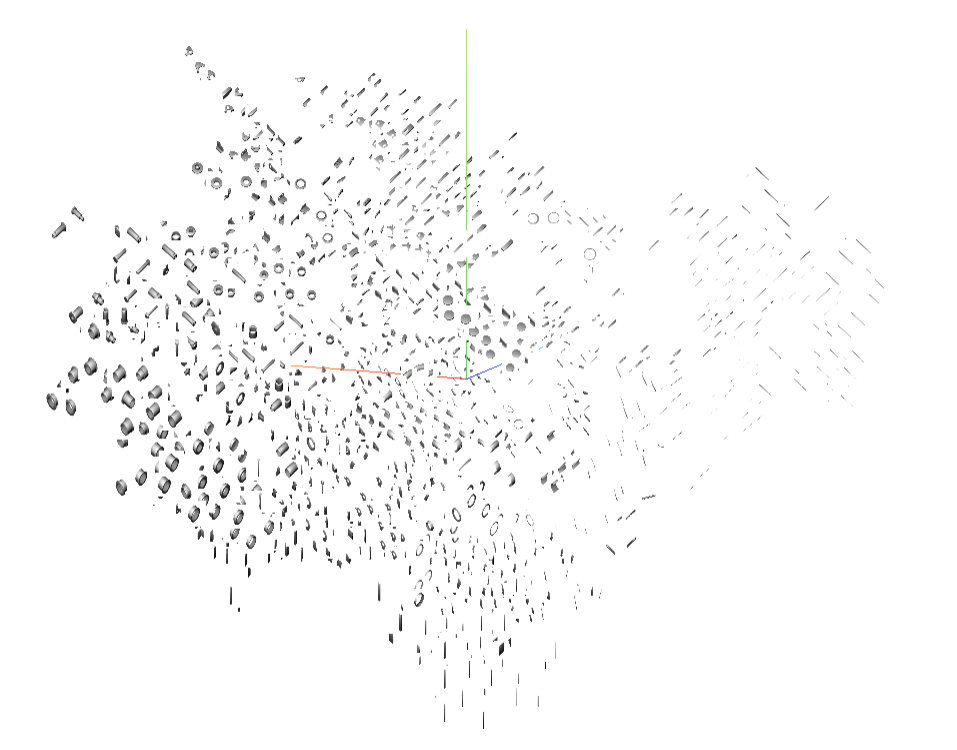
\includegraphics[width=0.7\columnwidth]{images/clusters_pca.png}
    \caption{PCA clustering of spherified sample embeddings.}
    \label{fig:pca_clusters}
\end{figure}

\begin{figure}[]
    \centering
    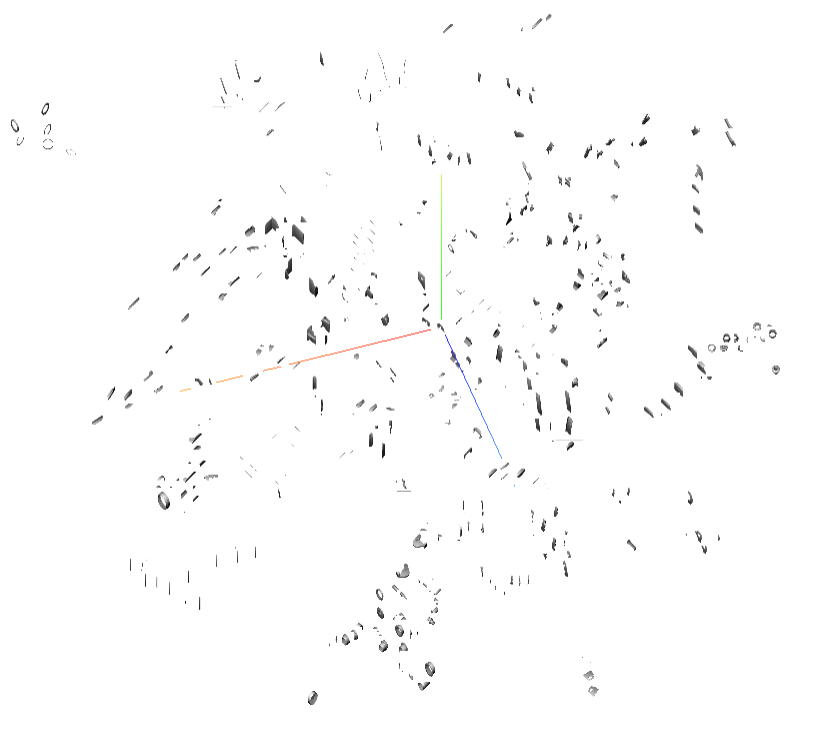
\includegraphics[width=0.7\columnwidth]{images/clusters_tsne.png}
    \caption{t-SNE clustering of spherified sample embeddings.}
    \label{fig:tsne_clusters}
\end{figure}

%%% Local Variables: 
%%% mode: latex
%%% TeX-master: "isae-report-template"
%%% End: 


\appendix
\label{sec:appendix}

\section{Triplets generation heuristics}
\label{sec:triplet-generation-heuristics}

\subsection{Triplets selection}

For each anchor data point, we fix a target distance, and a delta percentage.
We can in this way find a first data point which distance to the anchor data point is close to the fixed target distance.

Then, we can find a second data point which distance to the anchor data point is close to the fixed target distance \textbf{plus} a percentage of this target distance, defined by delta. We have to be careful not to propose the same data point here (especially working with small values).

The proposed triplet is the concatenation of these three data points. In the following, for simplicity, we will call these 3 data points respectively the anchor, the positive and the negative, even if the proposed negative can actually be the real positive (hard triplet).

This selection process is shown in \autoref{fig:triplet_generation}. 

\begin{figure}[]
    \centering
    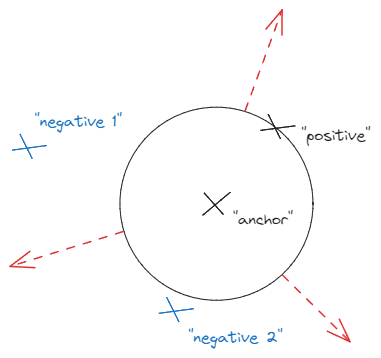
\includegraphics[width=0.4\columnwidth]{images/triplet_generation.png}
    \caption{Triplet selection process. An "anchor" point is selected, and a "positive" point is found at a fixed target distance. A "negative" point is then found at a distance defined by the target distance plus a delta percentage. How far is the negative point matters a lot. If negative 1 is chosen, the triplet will likely be easy to label, but will not bring a lot of value to the model. If negative 2 is chosen, the triplet will likely be hard to label (and thus skipped), but will bring a lot of value to the model.}
    \label{fig:triplet_generation}
\end{figure}

We initially used target distances uniformly distributed between 0.001 and 0.05, and delta uniformly distributed between 0.1 and 0.5.

These hyperparameters must be tuned according to the dataset. Iterative visual inspections were conducted to ensure that the triplets generated were relevant according to the properties defined in \autoref{sec:triplet-generation}.

\subsection{Triplets filtering}

Once our triplets are selected, we have to filter some triplets that do not bring enough value, or that will be too hard for the user to label.

\begin{enumerate}
    \item  Concatenation of the triplets found for each pair of parameters can lead to duplicate triplets -> Duplicated triplets are discarded.
    \item  It turns out that triplets with the same anchor and positive points share really similar negative point -> Duplicated (anchor, positive) triplets are discarded.
    \item Working with small target distances and deltas can lead to undesirable behaviours -> Triplets where the distance from the anchor to the positive $0$ are discarded. Triplets where the distance from the anchor to the positive is greater than the distance from the anchor to the negative are discarded.
    \item Sometimes, the positive and the negative data points turn out to be pretty similar -> Triplets where the relative distance from the positive to the negative is greater than a percentage of the distance from the anchor to the positive are discarded.
\end{enumerate}

All these filters aim at reducing as much as possible the amount of triplets that won't be labeled by the user.
\bibliographystyle{plain}
\bibliography{SFE_report}

\clearpage

%%%%%%%%%%%%%%%%
%%% Abstract %%%
%%%%%%%%%%%%%%%%

\thispagestyle{empty}

\vspace*{\fill}
\noindent\rule[2pt]{\textwidth}{0.5pt}\\
{\textbf{Résumé ---}}
Lorem ipsum dolor sit amet, consectetur adipiscing elit. Sed non risus. Suspendisse lectus tortor, dignissim sit amet, adipiscing nec, ultricies sed, dolor. Cras elementum ultrices diam. Maecenas ligula massa, varius a, semper congue, euismod non, mi. Proin porttitor, orci nec nonummy molestie, enim est eleifend mi, non fermentum diam nisl sit amet erat. Duis semper. Duis arcu massa, scelerisque vitae, consequat in, pretium a, enim. Pellentesque congue. Ut in risus volutpat libero pharetra tempor. Cras vestibulum bibendum augue. Praesent egestas leo in pede. Praesent blandit odio eu enim. Pellentesque sed dui ut augue blandit sodales. Vestibulum ante ipsum primis in faucibus orci luctus et ultrices posuere cubilia Curae; Aliquam nibh. Mauris ac mauris sed pede pellentesque fermentum. Maecenas adipiscing ante non diam sodales hendrerit. Ut velit mauris, egestas sed, gravida nec, ornare ut, mi. Aenean ut orci vel massa suscipit pulvinar. Nulla sollicitudin. Fusce varius, ligula non tempus aliquam, nunc turpis ullamcorper nibh, in tempus sapien eros vitae ligula. Pellentesque rhoncus nunc et augue. Integer id felis.

{\textbf{Mots clés :}}
Lorem ipsum dolor sit amet, consectetur adipiscing elit. Sed non risus. Suspendisse lectus tortor.
\\
\noindent\rule[2pt]{\textwidth}{0.5pt}
\begin{center}
  ISAE\\
  10, avenue Édouard Belin\\
  BP 54032\\
  31055 Toulouse CEDEX 4
\end{center}
\vspace*{\fill}

\end{document}